\section{The Morton Curve}
\subsection{Morton Keys}
\begin{frame}
    \frametitle{Morton Keys}
    2D cartesian coordinates in binary representation:
    \begin{equation}
        \left( x, y \right) = \left( \bb x_n \cdots x_2 x_1, \bb y_n \cdots
        y_2, y_1 \right)
    \end{equation}
    Interleaving and shuffeling their components yields the \textbf{Morton Key}
    of the coordinate pair $z$:
    \begin{equation}
        \begin{array} {c|c c c c c c c c c}
            x & & x_n & & x_{n-1} & \cdots & & x_2 & & x_1 \\
            y & y_n & & y_{n-1} & & \cdots & y_2 & & y_1 \\
            \hline
            z & y_n & x_n & y_{n-1} & x_{n-1} & \cdots & y_2 & x_2 & y_1 & x_1
        \end{array}
    \end{equation}
    \textbf{Example:}
    $\left( 5, 6 \right)=\left(\bb 0 1 0 1, \bb 0 1 1 0\right)$
    \begin{equation}
        \begin{array} {c|c c c c c c c c c}
            x & & 0 & & 1 & & 0 & & 1 \\
            y & 0 & & 1 & & 1 & & 0 \\
            \hline
            z & 0 & 0 & 1 & 1 & 1 & 0 & 0 & 1
        \end{array}
    \end{equation}
    $\implies\boxed{z=\bb00111001=\xx39=57}$
\end{frame}

\subsection{Morton Curve}
\begin{frame}
    \frametitle{Morton Curve}
    \textbf{Construction:}
    \begin{itemize}
        \item Calculate morton key $\forall \left(x, y\right)$ \\
        \item Sort them \\
        \item Draw a line from point to point in the order of the sorted morton
            keys
    \end{itemize}
    \textbf{Properties:}
    \begin{itemize}
        \item Space filling \\
        \item Proximity on the morton curve $\implies$ Spatial proximity
            ($\nLeftarrow$)
    \end{itemize}
\end{frame}

\begin{frame}
    \begin{figure}
        \centering
        \includegraphics[width=.8\textwidth]{Z-curve.png}
        \caption{General morton curve, source: Wikipedia}
    \end{figure}
\end{frame}

\begin{frame}
    \begin{figure}
        \centering
        \resizebox{.8\textwidth}{!}{%
            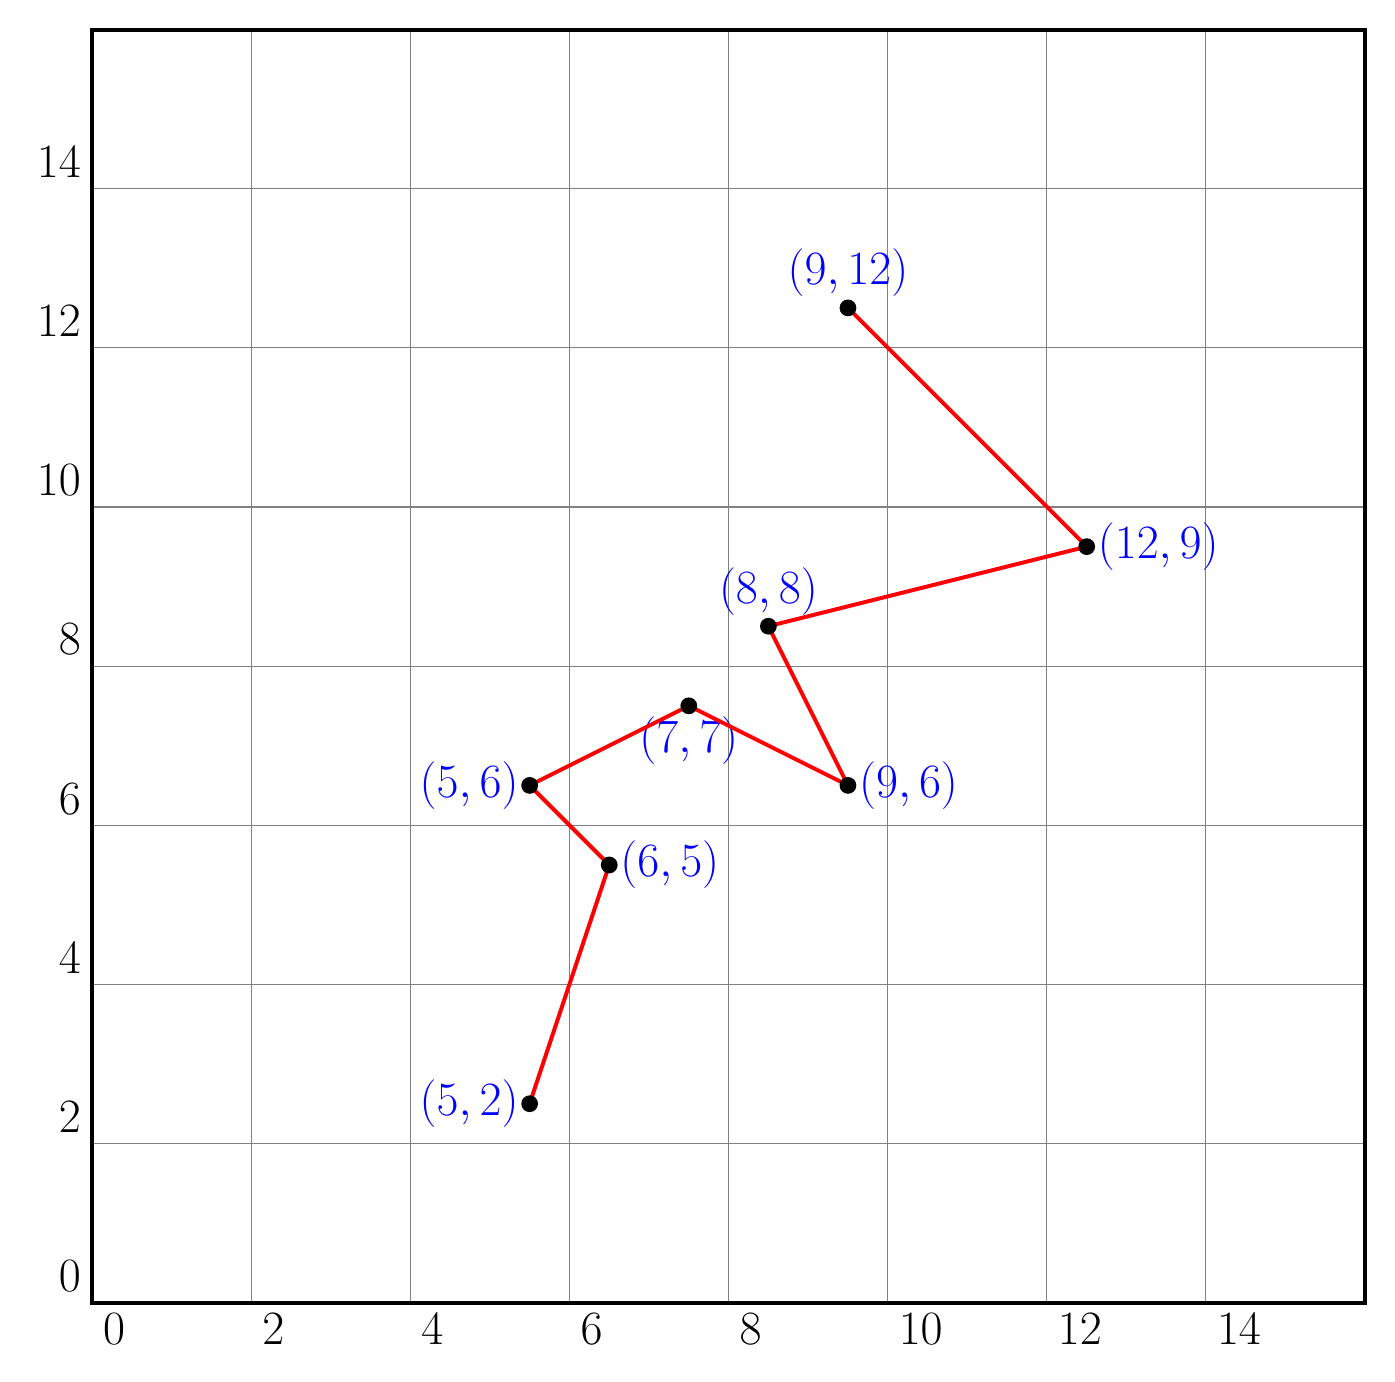
\begin{tikzpicture}[scale=\textwidth/12cm, line width=.5mm,
    morton/.style={every path/.style={draw=red}}]
    \def\A{\LARGE{\textcolor{blue}{$(5, 2)$}}}
    \def\B{\LARGE{\textcolor{blue}{$(6, 5)$}}}
    \def\C{\LARGE{\textcolor{blue}{$(5, 6)$}}}
    \def\D{\LARGE{\textcolor{blue}{$(7, 7)$}}}
    \def\E{\LARGE{\textcolor{blue}{$(9, 6)$}}}
    \def\F{\LARGE{\textcolor{blue}{$(8, 8)$}}}
    \def\G{\LARGE{\textcolor{blue}{$(12, 9)$}}}
    \def\H{\LARGE{\textcolor{blue}{$(9, 12)$}}}

    \draw[step=2cm,gray,thin] (0, 0) grid (16, 16);
    \draw (0, 0) rectangle (16, 16);

    \coordinate [label=left:\A] (A) at (5.5, 2.5);
    \coordinate [label=right:\B] (B) at (6.5, 5.5);
    \coordinate [label=left:\C] (C) at (5.5, 6.5);
    \coordinate [label=below:\D] (D) at (7.5, 7.5);
    \coordinate [label=right:\E] (E) at (9.5, 6.5);
    \coordinate [label=above:\F] (F) at (8.5, 8.5);
    \coordinate [label=right:\G] (G) at (12.5, 9.5);
    \coordinate [label=above:\H] (H) at (9.5, 12.5);

    \foreach \p in {0,2,...,14}{%
        \draw (0,\p) node[anchor=south east] {\LARGE{$\p$}};
        \draw (\p,0) node[anchor=north west] {\LARGE{$\p$}};
    }

    \begin{scope}[morton]
    \draw (A) -- (B);
    \draw (B) -- (C);
    \draw (C) -- (D);
    \draw (D) -- (E);
    \draw (E) -- (F);
    \draw (F) -- (G);
    \draw (G) -- (H);
    \end{scope}

    \foreach \point in {A, B, C, D, E, F, G, H}
        \fill [black] (\point) circle (3pt);
\end{tikzpicture}

% vim: set ff=unix tw=79 sw=4 ts=4 et ic ai :

        }
        \caption{Simple morton curve for small set of points}
    \end{figure}
\end{frame}

\subsection{Neighbours}
\begin{frame}
    \frametitle{Finding Neighbours on the Morton Curve}
    How does one find the neighbours of a given point based on its morton key?
    \\ (Here we are using 8-bit keys $\implies x, y = 0, \dots, 15 = 2^4-1$)
    \begin{align}
        \textrm{\textbf{left}}\left(z\right) =& \left(\left(\left(
            z \AND \bb01010101 \right) - 1 \right) \AND \bb01010101 \right)
            \nonumber \\
            &\;\,\OR \left( z \AND \bb10101010 \right)
    \end{align}
    \textbf{Example:} $\left( 5, 6 \right) = \bb00111001$
    \begin{align}
        \begin{array}{c c c}
            w :=& z \AND \bb01010101 &= \bb00010001 \\
            w :=& w - 1 &= \bb00010000 \\
            w :=& w \AND \bb01010101 &= \bb00010000 \\
            \tilde{w} :=& z \AND \bb10101010 &= \bb00101000 \\
            & w \OR \widetilde{w} &= \bb00111000
        \end{array} \\
        \begin{array}{c | c c c c c c c c}
            z & 0 & 0 & 1 & 1 & 1 & 0 & 0 & 0 \\
            \hline
            x & & 0 & & 1 & & 0 & & 0 \\
            y & 0 & & 1 & & 1 & & 0 \\
        \end{array}
        \implies \boxed{\textrm{left}\left(\left(5, 6\right)\right) =
        \left(4, 6\right)}
    \end{align}
\end{frame}

\begin{frame}
    \begin{align}
        \textrm{\textbf{right}}\left(z\right) =& \left(\left(\left(
            z \OR \bb10101010 \right) + 1 \right) \AND \bb01010101 \right)
            \nonumber \\
            &\;\,\OR \left( z \AND \bb10101010 \right)
    \end{align}
    \textbf{Example:} $\left( 5, 6 \right) = \bb00111001$
    \begin{align}
        \begin{array}{c c c}
            w :=& z \OR \bb10101010 &= \bb10111011 \\
            w :=& w + 1 &= \bb10111100 \\
            w :=& w \AND \bb01010101 &= \bb00010100 \\
            \tilde{w} :=& z \AND \bb10101010 &= \bb00101000 \\
            & w \OR \widetilde{w} &= \bb00111100
        \end{array} \\
        \begin{array}{c | c c c c c c c c}
            z & 0 & 0 & 1 & 1 & 1 & 1 & 0 & 0 \\
            \hline
            x & & 0 & & 1 & & 1 & & 0 \\
            y & 0 & & 1 & & 1 & & 0 \\
        \end{array}
        \implies \boxed{\textrm{left}\left(\left(5, 6\right)\right) =
        \left(6, 6\right)}
    \end{align}
\end{frame}

\begin{frame}
    \begin{align}
        \textrm{\textbf{top}}\left(z\right) =& \left(\left(\left(z \AND
        \bb10101010 \right) -1 \right) \AND \bb10101010 \right)
        \nonumber \\
        &\;\,\OR \left( z \AND
        \bb01010101 \right)
    \end{align}
    \begin{align}
        \textrm{\textbf{bottom}}\left(z\right) =& \left(\left(\left(z \OR
        \bb01010101 \right) +1 \right) \AND \bb10101010 \right)
        \nonumber \\
        &\;\,\OR \left( z \AND
        \bb01010101 \right)
    \end{align}
\end{frame}

% vim: set ff=unix tw=79 sw=4 ts=4 et ic ai :
